%%%%%%%%%%%%%%%%%%%%%%%%%%%%%%%%%%%%%%%%%%%%%%%%%%%%%%%%%%%%%%%%%%%%%%%%
%% Customizações do abnTeX2 (http://abnTeX2.googlecode.com)           %%
%% para a Universidade Estadual do Ceara - UECE                       %%
%%                                                                    %%
%% This work may be distributed and/or modified under the             %% 
%% conditions of the LaTeX Project Public License, either version 1.3 %%
%% of this license or (at your option) any later version.             %%
%% The latest version of this license is in                           %%
%%   http://www.latex-project.org/lppl.txt                            %%
%% and version 1.3 or later is part of all distributions of LaTeX     %%
%% version 2005/12/01 or later.                                       %%
%%                                                                    %%
%% This work has the LPPL maintenance status `maintained'.            %%
%%                                                                    %%
%% The Current Maintainer of this work is Thiago Nascimento           %%
%%                                                                    %%
%% Project available on: https://github.com/thiagodnf/uecetex2        %%
%%                                                                    %%
%% Further information about abnTeX2                                  %%
%% are available on http://abntex2.googlecode.com/                    %%
%%                                                                    %%
%%%%%%%%%%%%%%%%%%%%%%%%%%%%%%%%%%%%%%%%%%%%%%%%%%%%%%%%%%%%%%%%%%%%%%%%

%%%%%%%%%%%%%%%%%%%%%%%%%%%%%%%%%%%%%%%%%%%%%%%%%%%%%%%%%%%%%%%%%%%%%%%%
%% Customizações do abnTeX2 (http://abnTeX2.googlecode.com)           %%
%% para a Universidade Estadual do Ceara - UECE                       %%
%%                                                                    %%
%% This work may be distributed and/or modified under the             %% 
%% conditions of the LaTeX Project Public License, either version 1.3 %%
%% of this license or (at your option) any later version.             %%
%% The latest version of this license is in                           %%
%%   http://www.latex-project.org/lppl.txt                            %%
%% and version 1.3 or later is part of all distributions of LaTeX     %%
%% version 2005/12/01 or later.                                       %%
%%                                                                    %%
%% This work has the LPPL maintenance status `maintained'.            %%
%%                                                                    %%
%% The Current Maintainer of this work is Thiago Nascimento           %%
%%                                                                    %%
%% Project available on: https://github.com/thiagodnf/uecetex2        %%
%%                                                                    %%
%% Further information about abnTeX2                                  %%
%% are available on http://abntex2.googlecode.com/                    %%
%%                                                                    %%
%%%%%%%%%%%%%%%%%%%%%%%%%%%%%%%%%%%%%%%%%%%%%%%%%%%%%%%%%%%%%%%%%%%%%%%%

\documentclass[        
    a4paper,          % Tamanho da folha A4
    12pt,             % Tamanho da fonte 12pt
    chapter=TITLE,    % Todos os capitulos devem ter caixa alta
    section=TITLE,    % Todas as secoes devem ter caixa alta
    oneside,          % Usada para impressao em apenas uma face do papel
    english,          % Hifenizacoes em ingles
    french,           % Hifenizacoes em frances
    spanish,          % Hifenizacoes em espanhol
    brazil            % Ultimo idioma eh o idioma padrao do documento
]{abntex2}

% Importações de pacotes
\usepackage[alf, abnt-emphasize=bf, bibjustif, recuo=0cm, abnt-etal-cite=2, abnt-etal-list=0]{abntex2cite}  % Citações padrão ABNT
\usepackage[utf8]{inputenc}                         % Acentuação direta
\usepackage[T1]{fontenc}                            % Codificação da fonte em 8 bits
\usepackage{graphicx}                               % Inserir figuras
\usepackage{amsfonts, amssymb, amsmath}             % Fonte e símbolos matemáticos
\usepackage{booktabs}                               % Comandos para tabelas
\usepackage{verbatim}                               % Texto é interpretado como escrito no documento
\usepackage{multirow, array}                        % Múltiplas linhas e colunas em tabelas
\usepackage{indentfirst}                            % Endenta o primeiro parágrafo de cada seção.
\usepackage{microtype}                              % Para melhorias de justificação?
\usepackage[portuguese,ruled,lined]{algorithm2e}    % Escrever algoritmos
\usepackage{algorithmic}                            % Criar Algoritmos  
%\usepackage{float}                                  % Utilizado para criação de floats
\usepackage{amsgen}
\usepackage{lipsum}                                 % Usar a simulação de texto Lorem Ipsum
\usepackage{titlesec}                               % Permite alterar os títulos do documento
\usepackage{tocloft}                                % Permite alterar a formatação do Sumário
\usepackage{etoolbox}                               % Usado para alterar a fonte da Section no Sumário
\usepackage[nogroupskip,nonumberlist,acronym]{glossaries}                % Permite fazer o glossario
\usepackage{caption}                                % Altera o comportamento da tag caption

%\usepackage[bottom]{footmisc}                      % Mantém as notas de rodapé sempre na mesma posição
%\usepackage{times}                                 % Usa a fonte Times
\usepackage{mathptmx}                               % Usa a fonte Times New Roman										
%\usepackage{lmodern}                               % Usa a fonte Latin Modern
%\usepackage{subfig}                                % Posicionamento de figuras
%\usepackage{scalefnt}                              % Permite redimensionar tamanho da fonte
%\usepackage{color, colortbl}                       % Comandos de cores
%\usepackage{lscape}                                % Permite páginas em modo "paisagem"
%\usepackage{ae, aecompl}                           % Fontes de alta qualidade
%\usepackage{picinpar}                              % Dispor imagens em parágrafos
%\usepackage{latexsym}                              % Símbolos matemáticos
%\usepackage{upgreek}                               % Fonte letras gregas
\usepackage{appendix}                               % Gerar o apendice no final do documento
\usepackage{paracol}                                % Criar paragrafos sem identacao
\usepackage{lib/uecetex2}		                    % Biblioteca com as normas da UECE para trabalhos academicos
\usepackage{pdfpages}                               % Incluir PDF no documento

% Organiza e gera a lista de abreviaturas, simbolos e glossario
\makeglossaries

% Gera o Indice do documento
\makeindex

%%%%%%%%%%%%%%%%%%%%%%%%%%%%%%%%%%%%%%%%%%%%%%%%%%%%%
%%          Configuracoes do ueceTeX2              %%
%%%%%%%%%%%%%%%%%%%%%%%%%%%%%%%%%%%%%%%%%%%%%%%%%%%%%

% Opcoes disponiveis

%\trabalhoacademico{tccgraduacao}
%\trabalhoacademico{tccespecializacao}
\trabalhoacademico{dissertacao}
%\trabalhoacademico{tese}

% Define se o trabalho eh uma qualificacao
% Coloque 'nao' para versao final do trabalho

\ehqualificacao{nao}

% Remove as bordas vermelhas e verdes do PDF gerado
% Coloque 'sim' pare remover

\removerbordasdohyperlink{sim} 

% Adiciona a cor Azul a todos os hyperlinks

\cordohyperlink{nao}

%%%%%%%%%%%%%%%%%%%%%%%%%%%%%%%%%%%%%%%%%%%%%%%%%%%%%
%%          Informação sobre a IES                 %%
%%%%%%%%%%%%%%%%%%%%%%%%%%%%%%%%%%%%%%%%%%%%%%%%%%%%%

\ies{Universidade Estadual do Ceará}
\iessigla{UECE}
\centro{Centro de Ciências e Tecnologia}

%%%%%%%%%%%%%%%%%%%%%%%%%%%%%%%%%%%%%%%%%%%%%%%%%%%%%
%%        Informação para TCC de Graduacao         %%
%%%%%%%%%%%%%%%%%%%%%%%%%%%%%%%%%%%%%%%%%%%%%%%%%%%%%

\graduacaoem{Ciência da Computação}
\habilitacao{bacharel} % Pode colocar tambem 'licenciada'

%%%%%%%%%%%%%%%%%%%%%%%%%%%%%%%%%%%%%%%%%%%%%%%%%%%%%
%%     Informação para TCC de Especializacao       %%
%%%%%%%%%%%%%%%%%%%%%%%%%%%%%%%%%%%%%%%%%%%%%%%%%%%%%

\especializacaoem{Alfabetização de Crianças}

%%%%%%%%%%%%%%%%%%%%%%%%%%%%%%%%%%%%%%%%%%%%%%%%%%%%%
%%         Informação para Dissertacao             %%
%%%%%%%%%%%%%%%%%%%%%%%%%%%%%%%%%%%%%%%%%%%%%%%%%%%%%

\programamestrado{Programa de Pós-Graduação em Ciência da Computação}
\nomedomestrado{Mestrado Acadêmico em Ciência da Computação}
\mestreem{Ciência da Computação}
\areadeconcentracaomestrado{Ciência da Computação}

%%%%%%%%%%%%%%%%%%%%%%%%%%%%%%%%%%%%%%%%%%%%%%%%%%%%%
%%               Informação para Tese              %%
%%%%%%%%%%%%%%%%%%%%%%%%%%%%%%%%%%%%%%%%%%%%%%%%%%%%%

\programadoutorado{Programa de Pós-Graduação em Saúde Coletiva}
\nomedodoutorado{Doutorado em Saúde Coletiva}
\doutorem{Saúde Coletiva}
\areadeconcentracaodoutorado{Saúde Coletiva}

%%%%%%%%%%%%%%%%%%%%%%%%%%%%%%%%%%%%%%%%%%%%%%
%%  Informação relacionadas ao trabalho     %%
%%%%%%%%%%%%%%%%%%%%%%%%%%%%%%%%%%%%%%%%%%%%%%

\autor{Nome Sobrenome}
\titulo{Título do Trabalho}
\data{2014}
\local{Fortaleza -- Ceará}

% Exemplo: \dataaprovacao{01 de Janeiro de 2012}
\dataaprovacao{}

%%%%%%%%%%%%%%%%%%%%%%%%%%%%%%%%%%%%%%%%%%%%%
%%     Informação sobre o Orientador       %%
%%%%%%%%%%%%%%%%%%%%%%%%%%%%%%%%%%%%%%%%%%%%%

\orientador{Nome do seu Orientador}
\orientadories{Universidade Estadual do Ceará – UECE}
\orientadorcentro{Centro de Ciências e Tecnologia - CCT}
\orientadorfeminino{nao} % Coloque 'sim' se for do sexo feminino

%%%%%%%%%%%%%%%%%%%%%%%%%%%%%%%%%%%%%%%%%%%%%
%%      Informação sobre o Co-orientador   %%
%%%%%%%%%%%%%%%%%%%%%%%%%%%%%%%%%%%%%%%%%%%%%

% Deixe o nome do coorientador em branco para remover do documento

\coorientador{}
\coorientadories{Universidade Co-orientador - SIGLA}
\coorientadorcentro{Centro do Co-orientador - SIGLA}
\coorientadorfeminino{nao} % Coloque 'sim' se for do sexo feminino

%%%%%%%%%%%%%%%%%%%%%%%%%%%%%%%%%%%%%%%%%%%%%
%%      Informação sobre a banca           %%
%%%%%%%%%%%%%%%%%%%%%%%%%%%%%%%%%%%%%%%%%%%%%

% Atenção! Deixe o nome do membro da banca para remover da folha de aprovacao

% Exemplo de uso:
% \membrodabancadois{Prof. Dr. Fulano de Tal}
% \membrodabancadoisies{Universidade Estadual do Ceará - UECE}

\membrodabancadois{Membro da Banca Dois}
\membrodabancadoiscentro{Faculdade de Filosofia Dom Aureliano Matos – FAFIDAM}
\membrodabancadoisies{Universidade do Membro da Banca Dois - SIGLA}
\membrodabancatres{Membro da Banca Três}
\membrodabancatrescentro{Centro de Ciências e Tecnologia - CCT}
\membrodabancatresies{Universidade do Membro da Banca Três - SIGLA}
\membrodabancaquatro{Membro da Banca Quatro}
\membrodabancaquatrocentro{Centro de Ciências e Tecnologia - CCT}
\membrodabancaquatroies{Universidade do Membro da Banca Quatro - SIGLA}
\membrodabancacinco{Membro da Banca Cinco}
\membrodabancacincocentro{Teste}
\membrodabancacincoies{Universidade do Membro da Banca Cinco - SIGLA}
\membrodabancaseis{Membro da Banca Seis}
\membrodabancaseiscentro{}
\membrodabancaseisies{Universidade do Membro da Banca Seis - SIGLA}

\begin{document}	

	% Elementos pré-textuais
	\imprimircapa
	\imprimirfolhaderosto{}
	\imprimirfichacatalografica{elementos-pre-textuais/ficha-catalografica}
	\imprimirerrata{elementos-pre-textuais/errata}
	\imprimirfolhadeaprovacao
	\imprimirdedicatoria{elementos-pre-textuais/dedicatoria}
	\imprimiragradecimentos{elementos-pre-textuais/agradecimentos}
	\imprimirepigrafe{elementos-pre-textuais/epigrafe}
	\imprimirresumo{elementos-pre-textuais/resumo}
	\imprimirabstract{elementos-pre-textuais/abstract}
	\imprimirlistadeilustracoes
	\imprimirlistadetabelas
	\imprimirlistadequadros
	\imprimirlistadealgoritmos
	\imprimirlistadeabreviaturasesiglas	
	\imprimirlistadesimbolos{elementos-pre-textuais/lista-de-simbolos}   
	\imprimirsumario
	
	%Elementos textuais
	\textual
	\chapter{Introdução}
\label{chap:introducao}

\lipsum[2]

\begin{figure}[h!]
	\centering
	\Caption{\label{fig_mapa-5}Mapa conceitual do estudo da história e relações com o objeto de estudo}	
	\IBGEtab{}{
	    		\fbox{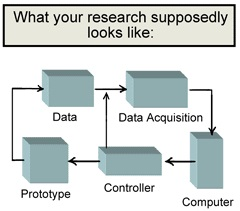
\includegraphics[width=8cm]{figuras/figura-1}}
	}{
		\Fonte{os autores}			
	}	
\end{figure}

\lipsum[2]
\lipsum[2]
\lipsum[2]

%\Gls{latex} e \gls{maths}
\Gls{ambiguidade}
\Gls{braile}
\Gls{coerencia}
\Gls{dialetos}
\Gls{elipse}
\Gls{locucao-adjetiva}
\Gls{modificadores}
\Gls{paronimos}
\Gls{sintese}
\Gls{borboleta}

\begin{figure}[h!]
	\centering
	\Caption{\label{fig_paradigma}Paradigma segundo processos que caracterizam a EFSFVS como Escola do SUS}	
	\IBGEtab{}{
		
\includegraphics[width=8cm]{figuras/figura-2}
	}{
		\Fonte{os autores}			
	}
\end{figure}

\lipsum[2]
\lipsum[2]

\section{Motivação}
\lipsum[2]
\lipsum[2]

\section{Objetivos}

\lipsum[2]

    \begin{table}[h!]
    	\centering	
    	\Caption{\label{tab:internal-3}Internal exon scores}    		
    	\IBGEtab{}{
        	\begin{tabular}{cll}
        		\toprule
        		Ranking & Exon Coverage & Splice Site Support\\
        		\midrule \midrule
        		E1 & Complete coverage by a single transcript & Both splice sites\\
        		E2 & Complete coverage by more than a single transcript & Both splice sites\\
        		E3 & Partial coverage & Both splice sites\\
        		E4 & Partial coverage & One splice site\\
        		E5 & Complete or partial coverage & No splice sites\\
        		E6 & No coverage & No splice sites\\
        		\bottomrule
        	\end{tabular}
    	}{
    		\Fonte{os autores}
    	}
    \end{table}

\lipsum[2]

\subsection{Objetivo Geral}

\lipsum[2]

\subsection{Objetivos Específicos}
	\lipsum[2]
	
	\begin{alineas}
		\item \lipsum[2]
		\item \lipsum[2]
		\begin{alineas}
			\item \lipsum[2]
			\item \lipsum[2]
		\end{alineas}
		\item \lipsum[2]	
	\end{alineas}
	
	\lipsum[2]
	
	\begin{table}[h!]	
		\centering
		\Caption{\label{tab:internal-1}Fatores de risco intermediários, não ajustados para a mortalidade infantil com malformação congênita, de acordo com as características maternas, Fortaleza, CE, BR, 2001 a 2010}		
		\IBGEtab{}{
    		\begin{tabular}{cll}
    			\hline
    			Ranking & Exon Coverage & Splice Site Support\\
    			\hline
    			E1 & Complete coverage by a single transcript & Both splice sites\\
    			E2 & Complete coverage by more than a single transcript & Both splice sites\\
    			E3 & Partial coverage & Both splice sites\\
    			E4 & Partial coverage & One splice site\\
    			E5 & Complete or partial coverage & No splice sites\\
    			E6 & No coverage & No splice sites\\
    			\hline
    		\end{tabular}
    	}{
			\Fonte{os autores}
		}
	\end{table}
	
	\lipsum[2]
	
\subsubsection{Objetivo Geral}
	\lipsum[2]
%	\cite{lamport1986latex} e \cite{wessberg2000real} e \cite{knuth} e \cite{lamport} e \cite{Maia2011} e \cite{mortalidade}
	
\subsubsection{Objetivo Geral}
	\lipsum[2]
	\acrlong{DATASUS},\acrlong{DNV},\acrlong{DO},\acrlong{ESF},\acrlong{IBGE},\acrlong{MFC},\acrlong{MI},\acrlong{MS},\acrlong{NV},\acrlong{ODM},\acrlong{OI},\acrlong{OMS},\acrlong{ONU},\acrlong{PNI},\acrlong{PSF},\acrlong{RIPSA},\acrlong{RN},\acrlong{SIM},\acrlong{SINASC},\acrlong{SUS},\acrlong{TMI},\acrlong{TMMFC}

\lipsum[2]
	\begin{algorithm}[h!]
		\Entrada{o proprio texto}
		\Saida{como escrever algoritmos com \LaTeX2e }
		\Inicio{
			inicializa\c{c}\~ao\;
			\Repita{fim do texto}{
				leia o atual\;
				\Se{entendeu}{
					vá para o próximo\;
					próximo se torna o atual\;}
				\Senao{volte ao início da seção\;}
			}
		}
		\caption{Exemplo de Algoritmo Versao 3}
	\end{algorithm}
	
\lipsum[2]	
	\chapter{Fundamentação Teórica}
\label{cap:fundamentacao-teorica}

Integer non lacinia magna. Aenean tempor lorem tellus, non sodales nisl commodo ut. Proin mattis placerat risus sit amet laoreet. Praesent sapien arcu, maximus ac fringilla efficitur, vulputate faucibus sem. Donec aliquet velit eros, sit amet elementum dolor pharetra eget. Integer eget mattis libero

\section{Fundamentação Teórica A}
\label{sec:fundamentacao-teorica-a}

\lipsum[10]

	\begin{figure}[h!]
		\centering
		\Caption{\label{fig:exemplo-1} Lorem ipsum dolor sit amet, consectetur adipiscing elit. Suspendisse commodo lectus et augue elementum varius.}	
		\UECEfig{}{
			\fbox{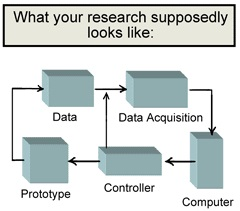
\includegraphics[width=8cm]{figuras/figura-1}}
		}{
			\Fonte{Elaborado pelo autor}
		}	
	\end{figure}
	
\lipsum[11]


\section{Fundamentação Teórica B}
\label{sec:fundamentacao-teorica-b}

Integer non lacinia magna. Aenean tempor lorem tellus, non sodales nisl commodo ut. Proin mattis placerat risus sit amet laoreet. Praesent sapien arcu, maximus ac fringilla efficitur, vulputate faucibus sem. Donec aliquet velit eros, sit amet elementum dolor pharetra eget. Integer eget mattis libero. Praesent ex velit, pulvinar at massa vel, fermentum dictum mauris. Ut feugiat accumsan augue, et ultrices ipsum euismod vitae

	\begin{figure}[h!]
		\centering
		\Caption{\label{fig:exemplo-2} Maecenas luctus augue odio, sed tincidunt nunc posuere nec}	
		\UECEfig{}{
			\fbox{
\includegraphics[width=8cm]{figuras/figura-2}}
		}{
			\Fonte{Elaborado pelo autor}			
		}	
	\end{figure}

Nunc ac pretium dui. Mauris aliquam dapibus nulla ac mattis. Aenean non tortor volutpat, varius lectus vitae, accumsan nibh. Cras pretium vestibulum enim, id ullamcorper tortor ultrices non. Integer sodales viverra faucibus. Curabitur at dui lacinia, rhoncus lacus at, blandit metus. Integer scelerisque non enim quis ornare.

\lipsum[13]

	\begin{table}[h!]	
		\centering
		\Caption{\label{tab:exemplo-1} Duis faucibus, enim quis tincidunt pellentesque, nisl leo varius nulla, vitae tempus dui mauris ac ante purus lorem}		
		\UECEtab{}{
			\begin{tabular}{cll}
				\toprule
				Ranking & Exon Coverage & Splice Site Support \\
				\midrule \midrule
				E1 & Complete coverage by a single transcript & Both splice sites\\
				E2 & Complete coverage by more than a single transcript & Both splice sites\\
				E3 & Partial coverage & Both splice sites\\
				E4 & Partial coverage & One splice site\\
				E5 & Complete or partial coverage & No splice sites\\
				E6 & No coverage & No splice sites\\
				\bottomrule
			\end{tabular}
		}{
		\Fonte{Elaborado pelo autor}
	}
	\end{table}

Duis faucibus, enim quis tincidunt pellentesque, nisl leo varius nulla, vitae tempus dui mauris ac ante. Quisque purus lorem, pharetra sit amet lobortis eu, vehicula vitae purus. Ut varius, erat nec vehicula elementum, risus est tempus justo, nec vulputate augue leo egestas metus.

	\begin{figure}[h!]
		\centering
		\Caption{\label{fig:exemplo-3} Ut posuere, ex quis sagittis auctor, magna massa euismod felis}	
		\UECEfig{}{
			\fbox{
\includegraphics[width=8cm]{figuras/figura-2}}
		}{
		\Fonte{Elaborado pelo autor}			
	}	
	\end{figure}

\lipsum[14]

	\begin{table}[h!]	
		\centering
		\Caption{\label{tab:exemplo-2} Etiam molestie, nulla a egestas aliquet, velit augue congue metus}		
		\UECEtab{}{
			\begin{tabular}{ccll}
				\toprule
				Quisque & pharetra & tempus & vulputate \\
				\midrule \midrule
				E1 & Complete coverage by a single transcript & Both splice sites\\
				E2 & Complete coverage by more than a single transcript & Both splice sites\\
				E3 & Partial coverage & Both splice sites & Both \\
				E4 & Partial coverage & One splice site & Both \\
				E5 & Complete or partial coverage & No splice sites & Both\\
				E6 & No coverage & No splice sites\\
				\bottomrule
			\end{tabular}
		}{
		\Fonte{Elaborado pelo autor}
	}
	\end{table}
	\chapter{Trabalhos Relacionados}
\label{cap:trabalhos-relacionados}

Integer non lacinia magna. Aenean tempor lorem tellus, non sodales nisl commodo ut. Proin mattis placerat risus sit amet laoreet. Praesent sapien arcu, maximus ac fringilla efficitur, vulputate faucibus sem. Donec aliquet velit eros, sit amet elementum dolor pharetra eget. Integer eget mattis libero

\section{Trabalho Relacionado A}
\label{sec:trabalho-relacionado-a}

\lipsum[10]

	\begin{figure}[h!]
		\centering
		\Caption{\label{fig:exemplo-1} Lorem ipsum dolor sit amet, consectetur adipiscing elit. Suspendisse commodo lectus et augue elementum varius.}	
		\UECEfig{}{
			\fbox{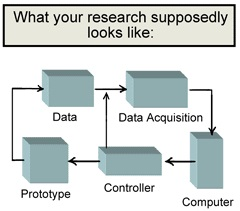
\includegraphics[width=8cm]{figuras/figura-1}}
		}{
			\Fonte{Elaborado pelo autor}
		}	
	\end{figure}
	
\lipsum[11]

\section{Trabalho Relacionado B}
\label{sec:trabalho-relacionado-b}

Integer non lacinia magna. Aenean tempor lorem tellus, non sodales nisl commodo ut. Proin mattis placerat risus sit amet laoreet. Praesent sapien arcu, maximus ac fringilla efficitur, vulputate faucibus sem. Donec aliquet velit eros, sit amet elementum dolor pharetra eget. Integer eget mattis libero. Praesent ex velit, pulvinar at massa vel, fermentum dictum mauris. Ut feugiat accumsan augue, et ultrices ipsum euismod vitae

	\begin{figure}[h!]
		\centering
		\Caption{\label{fig:exemplo-2} Maecenas luctus augue odio, sed tincidunt nunc posuere nec}	
		\UECEfig{}{
			\fbox{
\includegraphics[width=8cm]{figuras/figura-2}}
		}{
			\Fonte{Elaborado pelo autor}			
		}	
	\end{figure}

Nunc ac pretium dui. Mauris aliquam dapibus nulla ac mattis. Aenean non tortor volutpat, varius lectus vitae, accumsan nibh. Cras pretium vestibulum enim, id ullamcorper tortor ultrices non. Integer sodales viverra faucibus. Curabitur at dui lacinia, rhoncus lacus at, blandit metus. Integer scelerisque non enim quis ornare.

	\begin{quadro}[h!]	
		\centering
		\Caption{\label{qua:exemplo-1} Praesent ex velit, pulvinar at massa vel, fermentum dictum mauris. Ut feugiat accumsan augue}		
		\UECEqua{}{
			\begin{tabular}{|c|c|l|l|}
				\hline
				Quisque & pharetra & tempus & vulputate \\
				\hline
				E1 & Complete coverage by a single transcript & Both  & Complete\\
				\hline
				E2 & Complete coverage by more than & Both splice sites & Complete\\
				\hline
				E3 & Partial coverage & Both splice sites & Both \\				
				\hline
			\end{tabular}
		}{
			\Fonte{Elaborado pelo autor}
		}
	\end{quadro}
	
\lipsum[20]

	
	\begin{quadro}[h!]	
		\centering
		\Caption{\label{qua:exemplo-2} Duis faucibus, enim quis tincidunt pellentesque}		
		\UECEqua{}{
			\begin{tabular}{|c|c|}
				\hline
				Quisque & pharetra \\
				\hline
				E1 & Complete coverage by a single transcript \\
				\hline
				E2 & Complete coverage by more than \\
				\hline
				E3 & Partial coverage \\
				\hline
				E4 & Partial coverage \\
				\hline
				E5 & Partial coverage \\
				\hline
				E6 & Partial coverage \\
				\hline
				E7 & Partial coverage \\
				\hline
			\end{tabular}
		}{
			\Fonte{Elaborado pelo autor}
		}
	\end{quadro}

\lipsum[21]

Integer non lacinia magna. Aenean tempor lorem tellus, non sodales nisl commodo ut. Proin mattis placerat risus sit amet laoreet. Praesent sapien arcu, maximus ac fringilla efficitur, vulputate faucibus sem. Donec aliquet velit eros, sit amet elementum dolor pharetra eget. Integer eget mattis libero.
\Gls{ambiguidade}
\Gls{braile}
\Gls{coerencia}
\Gls{dialetos}
\Gls{elipse}
\Gls{locucao-adjetiva}
\Gls{modificadores}
\Gls{paronimos}
\Gls{sintese}
\Gls{borboleta}
	\chapter{Exemplo de Capítulos e Seções}
\label{chap:exemplo-de-capitulos-e-secoes}

Este capítulo descreve como você deve formatar os títulos do seu trabalho, ensinando também como você deve usá-los. O capítulo deve ser caixa alta, 12pt e com negrito. Para fazer um capítulo, você deve fazer:

\verb!\chapter{Escreva aqui o nome do Capítulo}!

\section{Seção Secundária}
As seções Secundárias deve ser caixa alta, 12pt e sem negrito. Para fazer uma seção Secundária, você deve fazer:

\verb!\section{Escreva aqui o nome da seção}!

\subsection{Seção Terciária}
As seções Terciárias deve ser caixa alta e baixa, 12pt e com negrito. Para fazer uma seção Terciária, você deve fazer:

\verb!\subsection{Escreva aqui o nome da seção}!

\subsubsection{Seção Quaternária}
As seções Quaternárias deve ser caixa alta e baixa, 12pt e sem negrito. Para fazer uma seção Quaternária, você deve fazer:

\verb!\subsubsection{Escreva aqui o nome da seção}!

\subsubsubsection{Seção Quinária}
As seções Quinárias deve ser caixa alta e baixa, 12pt e com itálico. Para fazer uma seção Quinária, você deve fazer:

\verb!\subsubsubsection{Escreva aqui o nome da seção}!
	\chapter{Conclusões e Trabalhos Futuros}
\label{chap:conclusoes-e-trabalhos-futuros}

\lipsum[2]
\lipsum[34]

\section{Contribuições do Trabalho}
\label{sec:contribuicoes-do-trabalho}

\lipsum[3]

\section{Limitações}
\label{sec:limitacoes}

\lipsum[4]

\section{Trabalhos Futuros}
\label{sec:trabalhos-futuros}

\lipsum[5]





	
	%Elementos pós-textuais	
	\bibliography{elementos-pos-textuais/referencias}
	\imprimirglossario	
	\imprimirapendices
		% Adicione aqui os apendices do seu trabalho
		\apendice{Lorem Ipsum}
\label{ap:lorem-ipsum}

\lipsum[1]
		\apendice{Modelo de Capa}
\label{ap:modelo-de-capa}

\lipsum[1]

		\apendice{Termo de Fiel Depositário}
\label{ap:termo-de-fiel-depositario}

\noindent \textbf{Pesquisa:} ANÁLISE DA MORTALIDADE INFANTIL COM MALFORMAÇÕES CONGÊNITAS.

\noindent Pelo presente instrumento que atende às exigências legais, a Sra. Maria Consuelo Martins Saraiva, ``fiel depositário'' com o cargo de Secretária Municipal de Saúde de Iracema, após ter tomado conhecimento do protocolo de pesquisa intitulado: ANÁLISE DA MORTALIDADE INFANTIL COM MALFORMAÇÕES CONGÊNITAS. Analisando a repercussão desse estudo no contexto da saúde pública e epidemiologia, autoriza Karla Maria da Silva Lima, enfermeira, aluna do Curso de Mestrado Acadêmico em Enfermagem da Universidade Estadual do Ceará (UECE), sob orientação do Prof. Dr. José Maria de Castro, da UECE, ter acesso aos bancos de dados do Sistema de Informação sobre Nascidos Vivos e do Sistema de Informação sobre Mortalidade da Secretaria Municipal de Saúde de Iracema, objeto deste estudo, e que se encontram sob sua total responsabilidade. Fica claro que o Fiel Depositário pode a qualquer momento retirar sua AUTORIZAÇÃO e ciente de que todas as informações prestadas tornar-se-ão confidenciais e guardadas por força de sigilo profissional, assegurando que os dados obtidos da pesquisa serão somente utilizados para estudo.	
	\imprimiranexos
		% Adicione aqui os anexos do seu trabalho
		\anexo{Dinâmica das classes sociais}
\label{an:dinamica-das-classes-sociais}

\index{AAA}
	\imprimirindice

\end{document}